\section{Methods and experimental design}
\subsection{Case I: parameter-efficient policy optimization}\label{sec:policy-methods}
\smallheading{Model and trainable representation}
The base model is \path{Qwen/Qwen2.5-0.5B}. Its pinned revision is\newline\code{060db6499f32faf8b98477b0a26969ef7d8b9987}.\cite{qwen} All seven runtime files were verified against the retained manifest, including the original weight SHA-256. ModelScope was the download transport; its \code{master} identifier was not treated as the pinned Hugging Face revision.

LoRA represents a correction to a frozen linear weight with two smaller matrices.\cite{lora,lorasurvey} For positive rank $r$ and column-vector input $\boldsymbol{x}\in\mathbb{R}^{d_{\mathrm{in}}}$,
\[
W\in\mathbb{R}^{d_{\mathrm{out}}\times d_{\mathrm{in}}},\qquad
A\in\mathbb{R}^{r\times d_{\mathrm{in}}},\qquad
B\in\mathbb{R}^{d_{\mathrm{out}}\times r}.
\]
\begin{align}
\Delta W&=\frac{\alpha}{r}BA,\nonumber\\
\boldsymbol{y}&=W\boldsymbol{x}+\boldsymbol{b}
+\frac{\alpha}{r}BA\boldsymbol{x}.\label{eq:lora}
\end{align}
The adapter adds $r(d_{\mathrm{in}}+d_{\mathrm{out}})$ parameters rather than updating all $d_{\mathrm{in}}d_{\mathrm{out}}$ elements of $W$. This is a trainable-parameter comparison, not an estimate of total memory savings: the base model still participates in forward and backward computation.

\par\noindent\begin{minipage}{\linewidth}
\begin{center}
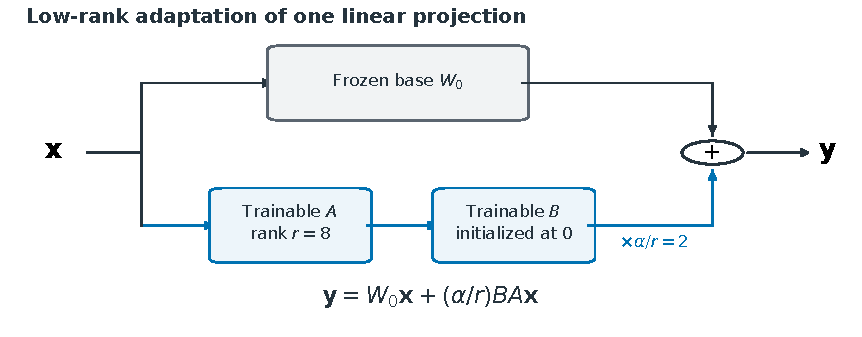
\includegraphics[width=146mm]{../../figures/lora_mechanism.pdf}
\end{center}
\figcaption{fig:lora}{A frozen linear transformation and its low-rank correction. Initializing $B$ to zero preserves the initial output; a nonzero initialization of $A$ permits learning. Inference merging incorporates the correction into $W$ and bypasses the separate branch.}
\end{minipage}\par


For row-batched PyTorch input $X$, Equation~\eqref{eq:lora} becomes
\begin{equation}
Y=XW^{\mathsf T}+\boldsymbol{1}\boldsymbol{b}^{\mathsf T}
+\frac{\alpha}{r}XA^{\mathsf T}B^{\mathsf T}.
\end{equation}
During training, dropout applies only to the adapter input. The equivalence used for merging is evaluated with dropout disabled. Merging performs $W\leftarrow W+\Delta W$ once; an explicit flag prevents adding the correction twice. The manual implementation and its tests are documented in Appendix~\ref{app:implementation}.

\smallheading{Learning rate and batch rationale}
Learning rate sets the scale of an optimizer update. A large value can accelerate initial fitting but destabilize optimization; a smaller value can leave the model under-adapted within a short budget. LoRA's factorized update makes rank, scaling and target modules part of this choice. An empirical analysis reports settings in which LoRA benefits from substantially higher learning rates than full fine-tuning and in which large batches widen the performance gap.\cite{lorablog} Those findings motivate careful tuning, rather than a universal multiplier.

Batch size also changes the number and variability of updates. Without accumulation, 1,024 examples yield 128 updates at batch 8 and 16 at batch 64. A comparison must therefore state whether data volume, update count or compute is held fixed. Here the effective training batch is 8, assembled from microbatches of 1 to limit memory. The Actor/Critic learning rates are $10^{-5}$ and $5\times10^{-5}$. They are fixed starting values; no sweep establishes their optimality.

\smallheading{PPO, value estimation and the reference policy}
OpenRLHF v0.6.0 is fixed to commit \code{bfa85f6fa8cd6214707f93883fac5d08334f4f06}.\cite{openrlhf} The Actor generates responses, the Critic predicts return, and a frozen initial policy provides the reference distribution. A local HTTP reward service grades arithmetic correctness, avoiding a separately trained reward model.

The clipped PPO objective is maximized:\cite{ppo}
\begin{align}
\rho_t(\theta)&=
\frac{\pi_{\theta}(a_t\mid s_t)}{\pi_{\mathrm{old}}(a_t\mid s_t)},\\
J_{\mathrm{clip}}(\theta)&=
\mathbb{E}_t\!\left[
\min\left(\rho_t(\theta)\widehat A_t,\,
\operatorname{clip}(\rho_t(\theta),1-\epsilon,1+\epsilon)\widehat A_t\right)
\right].\label{eq:ppo}
\end{align}
Here $s_t$ is the text prefix, $a_t$ the next token and $\pi_{\mathrm{old}}$ the policy used to collect the rollout. PPO clipping reduces the incentive for an excessive change; it does not strictly bound every update. The implementation minimizes the negative objective, so a signed Actor loss cannot be read as an accuracy measure.

Generalized advantage estimation (GAE) uses the Critic to form
\begin{equation}
\delta_t=\widetilde r_t+\gamma V_\phi(s_{t+1})-V_\phi(s_t),\qquad
\widehat A_t=\sum_{\ell=0}^{T-t-1}(\gamma\lambda)^\ell\delta_{t+\ell},
\end{equation}
with terminal handling supplied by the framework. The shaped reward $\widetilde r_t$ includes the reference-policy KL penalty. This reference differs from the rollout policy in the ratio $\rho_t$: one anchors behavior to the pretrained model, while the other controls an update relative to collected samples.

\par\noindent\begin{minipage}{\linewidth}
\tabcaption{tab:policy-settings}{Fixed settings of the successful policy-learning experiment. A rollout batch is not an optimizer-update count.}
\begin{tabularx}{\linewidth}{@{}P{53mm}Y@{}}
\toprule
\tablehead Setting & Value\\
\midrule
Model / hardware & Qwen2.5-0.5B; one NVIDIA A10; native BF16; ZeRO-2\\
Actor / Critic adapters & $r=8$, $\alpha=16$, dropout $=0$\\
Target projections & q/k/v/o and gate/up/down; Critic also adapts \code{score}\\
Actor / Critic learning rates & $10^{-5}$ / $5\times10^{-5}$; warmup ratio 0.03\\
Rollout / effective train batch & 16 / 8; both microbatches 1\\
PPO / reference regularization & $\epsilon=0.2$; value clip 0.2; initial KL coefficient 0.01\\
GAE / discount & $\lambda=0.95$; $\gamma=1$\\
Training budget & 512 prompts; one episode, one epoch; 32 rollout batches\\
Length / generation & Prompt limit 192; output limit 32 tokens; sampled training responses\\
Seed / memory & Seed 1234; gradient checkpointing\\
\bottomrule
\end{tabularx}
\end{minipage}\par


The budget nominally gives two effective updates per rollout, or 64 per network. Recorded curves use the 32 rollout-batch indices. The Critic includes a LoRA correction on \code{score} because PEFT freezes non-adapter weights; a frozen, unadapted value head would not match the intended configuration.

\smallheading{Data, scoring and paired evaluation}
With seed 1234, the data generator selects 512 training pairs and 128 disjoint validation pairs from $0\le a\le b<50$. Swapped-addend equivalents cannot cross the split. The two examples present in every prompt are excluded from both sets.

Reward is 1 when the first generated line is an integer equal to the sum, and 0 otherwise. Optional sign and horizontal whitespace are allowed; later lines are ignored. The reward service verifies and removes the complete prompt prefix and known padding/end tokens before scoring, preventing prompt examples from earning reward. This metric measures \emph{first-line integer accuracy}; it does not require the model to stop after one answer.

Before and after PPO, the same 128 questions are decoded greedily with a 32-token maximum in BF16. Scores are recomputed from saved responses. An earlier answer-tag rule was revised after observing validation responses, so this split is development validation rather than an untouched final test set.

\subsection{Case II: LLM-guided program search}\label{sec:program-methods}
LLM4AD\_Next, also branded OpenLoopX, searches over executable algorithms.\cite{llm4ad,architecture} An LLM proposes a modification, a Coder implements it within allowed evolution blocks, and a separate Evaluator executes the candidate under fixed constraints. The Orchestrator selects survivors and controls migration and stopping. These roles can share a model; they are not necessarily separately trained agents. Unlike the first case, this search changes program source rather than updating the LLM's weights.

\par\noindent\begin{minipage}{\linewidth}
\begin{center}
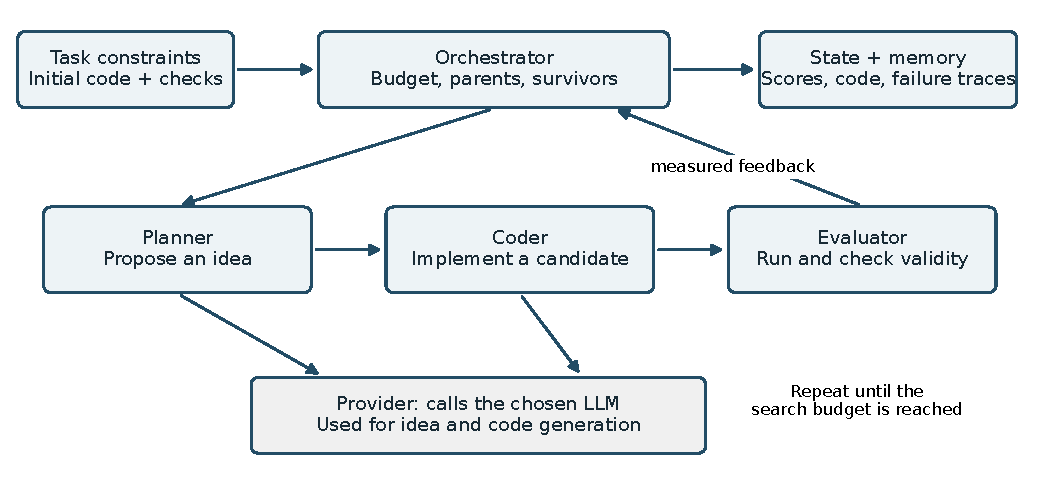
\includegraphics[width=166mm]{../../program_search/figures/framework.pdf}
\end{center}
\figcaption{fig:framework}{The platform's proposal--code--evaluation loop, reconstructed from the pinned architecture and data-flow documentation. The diagram explains component responsibilities and is not a screenshot of an executed task.}
\end{minipage}\par


A complete iteration records the parent program, proposed change, resulting source, score and error information. Island-based search maintains separate populations and periodically exchanges candidates; memory can supply prior solutions or failure explanations.\cite{dataflow,islands,memory} These facilities define possible feedback paths. Their effectiveness must be evaluated from the actual run rather than inferred from their availability.

\smallheading{Objective and fixed geometric constraints}
The selected AlphaEvolve mathematics template requires exactly 26 circles inside the unit square.\cite{benchmark,circle} For center $\boldsymbol c_i=(x_i,y_i)$ and radius $r_i$,
\begin{align}
\max_{\{\boldsymbol c_i,r_i\}_{i=1}^{26}}\quad&
S=\sum_{i=1}^{26}r_i,\label{eq:circle-objective}\\
\text{subject to}\quad&
r_i\ge0,\quad r_i\le x_i\le1-r_i,\quad r_i\le y_i\le1-r_i,\label{eq:circle-boundary}\\
&\|\boldsymbol c_i-\boldsymbol c_j\|_2\ge r_i+r_j\quad(i<j).\label{eq:circle-pairs}
\end{align}
The objective is the sum of radii, not area coverage. The evaluator also requires finite arrays of shapes $(26,2)$ and $(26,)$. Zero-radius circles are permitted. Visual plausibility does not replace these checks.

The official initial constructor was executed locally and accepted by the unchanged geometry-validation method extracted from the evaluator. Its sum was $0.9597642169962063$. This is a preparation measurement, not an online starting score for the later search. The initial geometry and selected program's local reproduction are shown separately from the online trajectory in Section~\ref{sec:program-results}.

\smallheading{Saved search design and observed execution}
The model was \emph{deepseek-v4-flash}, as reported by the platform. The online experiment ran on 31 October 2026. The revised task started at 12:38:01 (UTC+08:00); its final exported workspace was captured at 13:22:05, after which the task was manually stopped.

\par\noindent\begin{minipage}{\linewidth}
\tabcaption{tab:search-settings}{Saved search settings and actual stopping condition. A configured budget is not a count of completed evaluations.}
\begin{tabularx}{\linewidth}{@{}P{58mm}Y@{}}
\toprule
\tablehead Setting & Saved value / actual observation\\
\midrule
Task / seed & 26-circle construction; seed 42\\
Population design & 2 islands; initial target 2 candidates per island\\
Evolution / migration & Target 2 generations; migration interval 1, ring topology\\
Selection & Tournament parent selection; truncation survival\\
Variation & Mutation rate 0.3; crossover rate 0.5; elite ratio 0.2\\
LLM requests & At most 2 concurrent; Coder temperature 0.7\\
Request limits & Coder output ceiling 32,768; saved context limit 8,192\\
Evaluation & Original geometry objective; no evaluator retries\\
Memory & Extraction disabled in saved configuration\\
Actual stopping & Generation 1 completed; generation 2 started; manual stop after export\\
\bottomrule
\end{tabularx}
\end{minipage}\par


The saved YAML records the revised output ceiling (Appendix~\ref{app:platform}). Although memory extraction was disabled, the runtime still logged evaluation-trace embedding. The study does not infer that every memory-related operation was absent. This short demonstration is distinct from the repository's much larger published benchmark.

The explanatory source study uses repository commit \code{dfde353e753e9021fffe88b5b034bf0c84d90b60}. The hosted service may run another revision. Original exports remain in local archival storage; the public subset preserves the candidate and numerical evidence. Local verification uses the unchanged exported geometry method. Local figures retain saved centers and radii with equal axis scaling.
